\documentclass[a4paper,11pt]{article} % The document class with options

\usepackage[margin=1in]{geometry}
\usepackage{newtxtext,newtxmath}
\usepackage[T1]{fontenc}
\usepackage{amsmath}
\usepackage{amsfonts}
\usepackage{microtype}
\usepackage{graphicx}
% chktex-file 3
% chktex-file 18
% chktex-file 36
% chktex-file 44

\begin{document}
\setlength{\parskip}{1em} 
\setlength{\parindent}{0pt}
\newcommand{\vect}[1]{\mathbf{#1}}

\title{MECH 503 LAMMPS Project Report}
\author{Jincong Li \\ 60539939}
\date{\today}
\maketitle

\section*{Introduction}
Elastic constants are pivotal in understanding materials' responses to external forces, 
providing insights into stiffness and stability. This report delves into the nuances of these relationships 
across a spectrum of material types, including those classified as transversely isotropic and cubic symmetric.

%\subsection*{Isotropic materials} Isotropic materials are characterized by consistent mechanical properties in all directions, the stress-strain relationship adheres to the well-established Hooke's Law, articulated as:

%\[
%\sigma_{ij} = C_{ijkl}\varepsilon_{kl}
%\]

%Here, \(\sigma_{ij}\) represents the stress tensor, \(\varepsilon_{kl}\) denotes the strain tensor, and \(C_{ijkl}\) is the elastic stiffness tensor. Within the realm of isotropic materials, the stiffness tensor can be further simplified to:

%\[
%C_{ijkl} = \lambda\delta_{ij}\delta_{kl} + \mu(\delta_{ik}\delta_{jl} + \delta_{il}\delta_{jk})
%\]

%where \(\lambda\) and \(\mu\) are the Lamé constants, and \(\delta_{ij}\) is the Kronecker delta, encapsulating the essence of isotropic material behavior.

%\subsection*{Orthotropic materials} Orthotropic materials distinguished by unique mechanical properties along three orthogonal axes, the stress-strain equation becomes considerably more intricate, involving a fourth-order elastic stiffness tensor. Despite the potential for 81 components within this tensor, symmetries reduce the count of independent material constants to 21, illustrating the complexity inherent to orthotropic materials.

\subsection*{Transversely isotropic materials} Transversely isotropic materialsexhibit distinct properties along one axis as compared to the other two orthogonal directions. An exemplar of such materials is hexagonal close-packed (HCP) crystals, where the stress-strain relationship is characterized by a reduced form of the elastic stiffness matrix, symbolizing the specialized behavior of transversely isotropic substances.

\subsection*{Cubic symmetric materials} Cubic symmetric materials including face-centered cubic (FCC) and body-centered cubic (BCC) metals, showcase identical properties across all axes. Their behavior is succinctly captured by a constitutive law that is parameterizable by merely three material constants, simplifying the elastic stiffness matrix and highlighting the uniformity of cubic symmetric materials.

The exploration of these material types and their stress-strain relations provides a comprehensive overview of the mechanical behavior of materials under load, serving as a crucial foundation for predicting and analyzing the performance of engineering structures.

\subsection*{LAMMPS} With the advancement of molecular dynamics 
(MD) simulations, notably through the Large-scale Atomic/Molecular Massively Parallel Simulator
(LAMMPS), researchers can now predict these constants with high precision, bypassing the 
limitations of traditional experimental methods.

This study leverages LAMMPS to compute the elastic constant tensor for four 
materials: hexagonal close-packed magnesium (hcp-Mg), face-centered cubic aluminum 
(fcc-Al), body-centered cubic tungsten (bcc-W), and a novel face-centered cubic 
high-entropy alloy (HEA) consisting of nickel, iron, chromium, and cobalt. 
These materials are selected for their diverse applications, from aerospace to 
high-temperature environments. The focus is on examining the convergence of
the elastic constant tensor as a function of the finite difference displacement 
variable, "up" across a range from 0.01 to 0.0000001. This analysis is crucial for
validating the accuracy of our simulations against experimental and other 
computational data, providing a foundation for further exploration in materials science.
For HEA,  finite difference displacement 
variable, "up" is set to be $1e-6$, and the components of the elastic constant tensor are examined across different random lattice structures.

\section*{Methology}
\subsection*{Simulation Setup}
The molecular dynamics simulations were conducted using LAMMPS, focusing on four materials: hcp-Mg, fcc-Al, bcc-W, and an equiatomic high-entropy alloy of Ni, Fe, Cr, Co. For the high-entropy alloy, a Matlab script \texttt{make\_fcc\_random\_cell.m} was utilized to generate ten random FCC cells, ensuring a diverse representation of the alloy's microstructure. These cells were input into LAMMPS using the \texttt{read\_data} command.
Note that some components are omitted in the plots since they are essentially zero.
\subsection*{Potential Models}
Interaction potentials were chosen based on their ability to accurately represent each material's physics:
\begin{itemize}
    \item hcp-Mg, fcc-Al, and bcc-W: Embedded Atom Method (EAM) potentials were employed, sourced from literature where parameters have been validated against experimental and \textit{ab initio} data.
    \item High-Entropy Alloy: The \texttt{eam/alloy} pair style was used with parameters from a comprehensive study ensuring the representation of complex multi-element interactions.
\end{itemize}
The lattice parameter for each material is provided in the following table 1. Notice that for the HEA, the lattice is random generated by the provided MATLAB file and the reference pair style and coefficients are obtained from NIST[3].
\begin{table}[ht]
    \caption{Materials, Lattice Format and Parameter(a) }
    \centering
    \begin{tabular}{|l|c|c|}
        \hline
        Material & Lattice &a \\
        \hline   
        Aluminium (Al) & FCC & 4.05[1] \\
        Magnesiumg (Mg)& HCP & 3.21[2]\\
        Tungsten (W) & BCC & 3.165[1]\\
        HEA & random generate by MATLAB code & 4.093[3] \\
        \hline
    \end{tabular}
\end{table}

\subsection*{Finite Difference Parameter Analysis}
The elastic constant tensor's sensitivity to the finite difference displacement variable ``up'' was investigated by varying ``up'' between 0.01 to 0.0000001. This range was selected to encompass a broad spectrum of potential physical responses, enabling an assessment of convergence behavior. The analysis involved incrementally displacing atoms in the simulation cell and measuring the resultant stress, with elastic constants derived from the stress-strain relationship.

\subsection*{Data Processing and Analysis}
Post-simulation, the output data were processed using MATLAB scripts. Convergence plots were generated for each material, highlighting how the calculated elastic constants stabilize as ``up'' decreases. Special attention was given to the high-entropy alloy, considering the random nature of its structure.

\subsection*{Comparison with Existing Data}
The obtained elastic constants were compared to available experimental data and previous computational studies, such as those by Mishin et al., for validation purposes. This comparison aimed to assess the accuracy of the MD simulations conducted in this study and to elucidate the potential impact of the chosen potentials and simulation parameters on the results.

\section*{Result}
For Al, Mg, and W, the convergence plots for components of the elastic constant tensor are presebted below from figure 1 to figure 3. As one could observe, all the components converge to a stable value with the decrease of the scale of the finite difference parameter ``up''. The comparision between the final values with the reference values will be conducted later.
\begin{figure}[ht]
    \centering
    \includegraphics[width=1.1\textwidth]{Al.png}
    \caption{Convergence for Components of the Elastic Constant Tensor for fcc Al}
\end{figure}

\begin{figure}[ht]
    \centering
    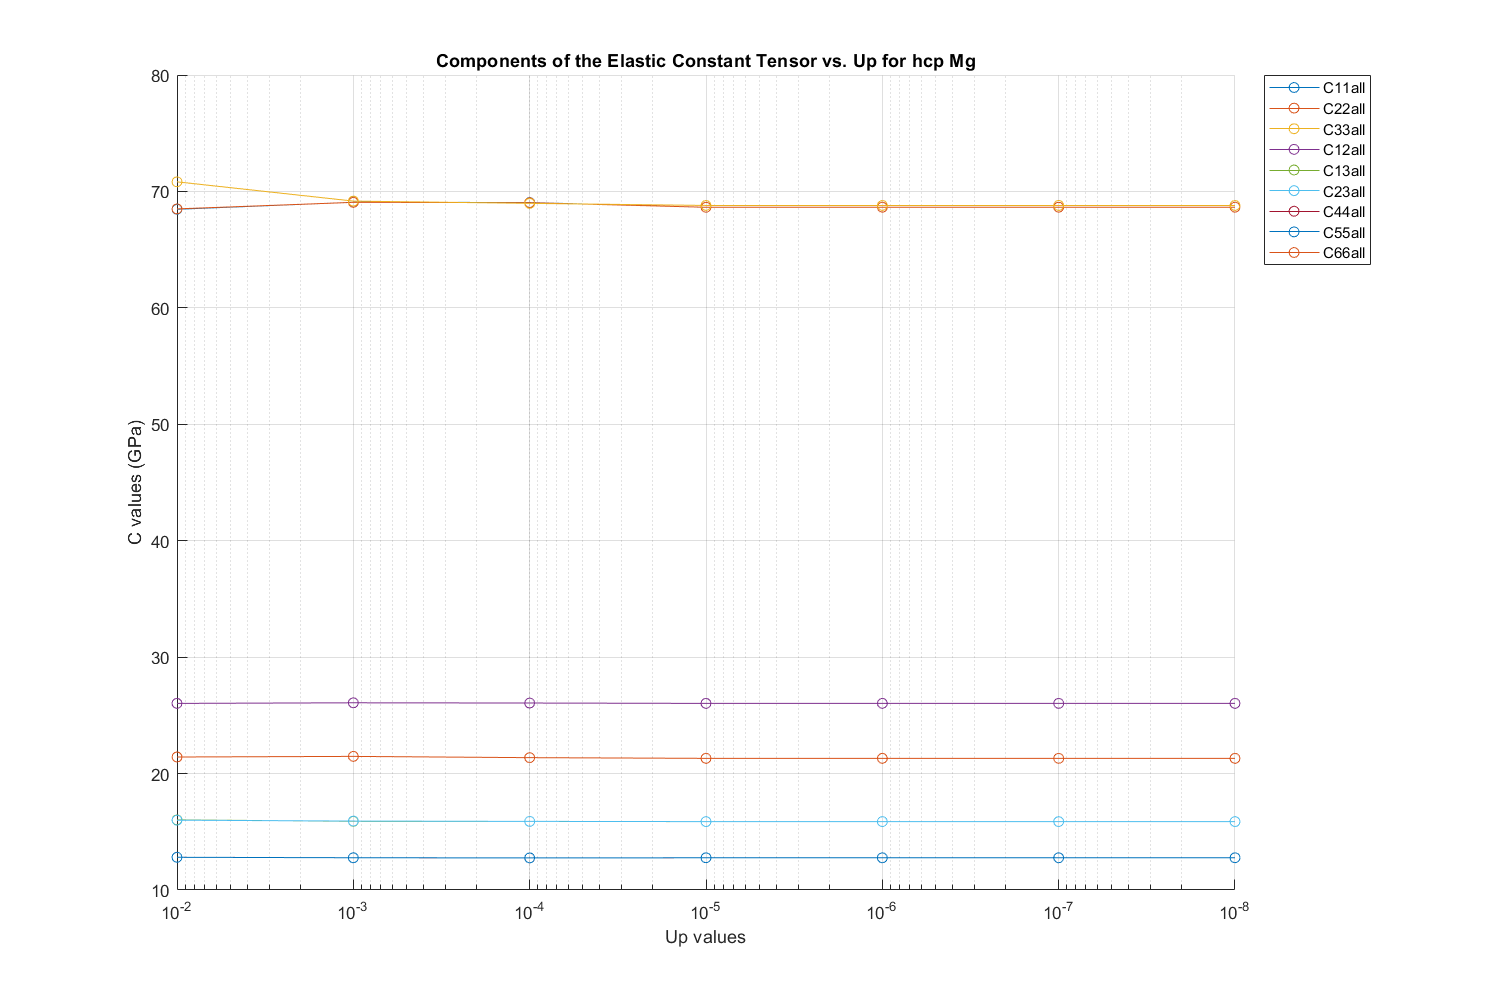
\includegraphics[width=1.1\textwidth]{Mg.png}
    \caption{Convergence for Components of the Elastic Constant Tensor for hcp Mg}
\end{figure}

\begin{figure}[ht]
    \centering
    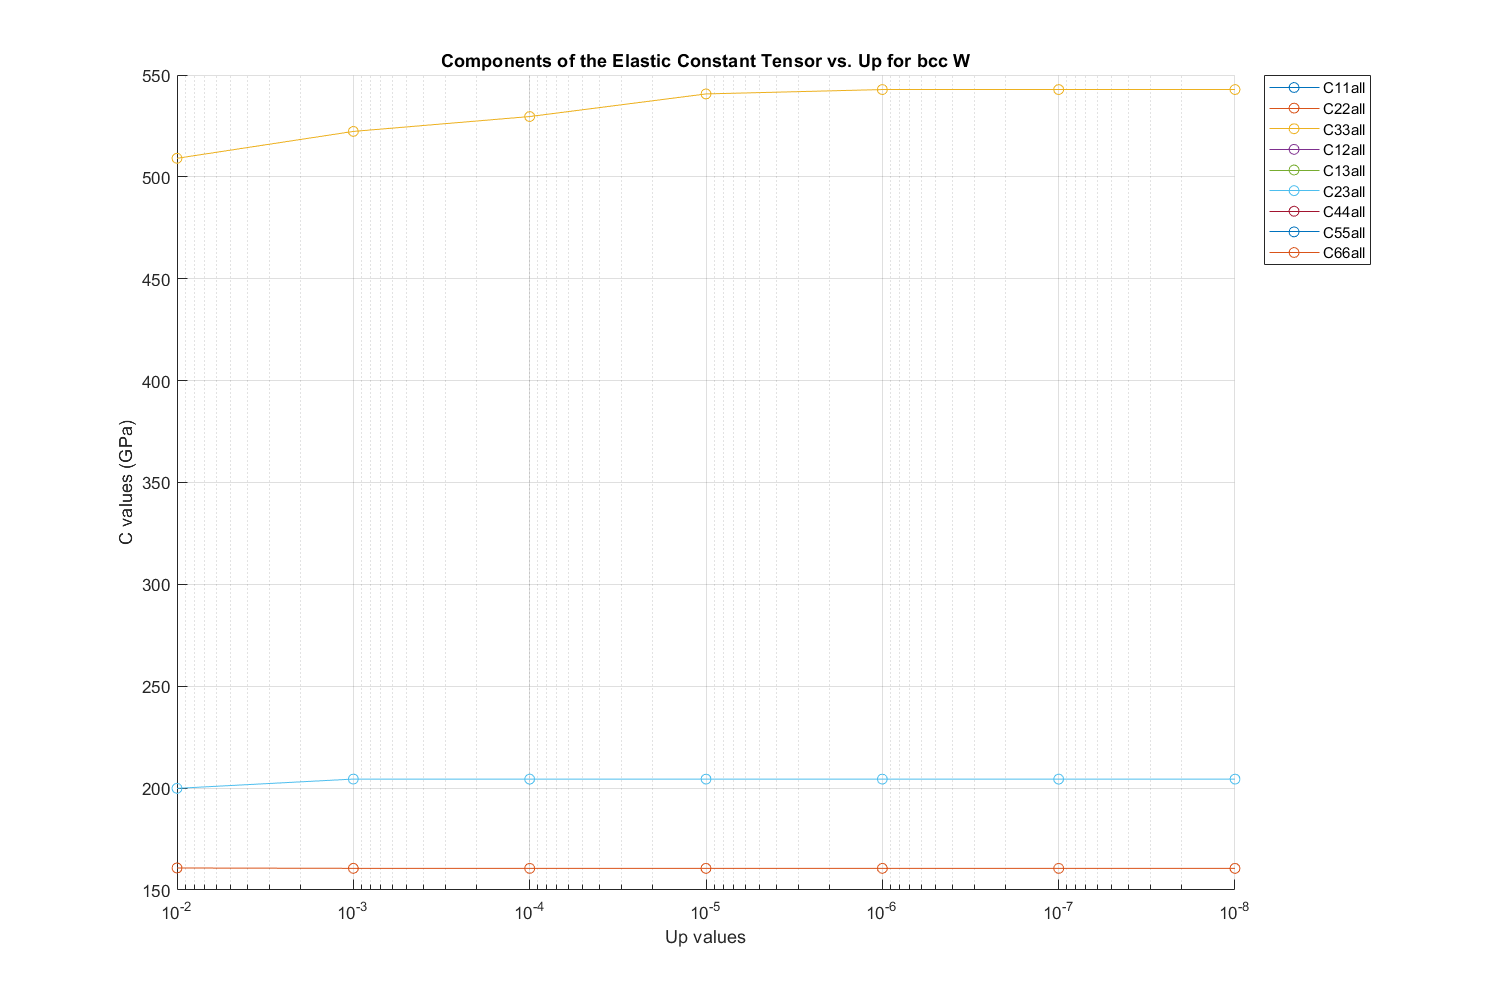
\includegraphics[width=1.1\textwidth]{W.png}
    \caption{Convergence for Components of the Elastic Constant Tensor for bcc W}
\end{figure}
\clearpage
\subsection*{Validation}
\begin{table}[H]
\centering
\begin{tabular}{|c|c|c|c|c|c|c|c|c|c|}
\hline
File Number C11all & C22all & C33all & C12all & C13all & C23all & C44all & C55all & C66all \\
\hline
1 & 113.39 & 113.39 & 113.39 & 61.04 & 61.04 & 61.04 & 31.70 & 31.70 & 31.70 \\
\hline
2 & 113.76 & 113.76 & 113.76 & 61.51 & 61.51 & 61.51 & 31.60 & 31.60 & 31.60 \\
\hline
3 & 113.79 & 113.79 & 113.79 & 61.55 & 61.55 & 61.55 & 31.59 & 31.59 & 31.59 \\
\hline
4 & 113.80 & 113.80 & 113.80 & 61.55 & 61.55 & 61.55 & 31.59 & 31.59 & 31.59 \\
\hline
5 & 113.80 & 113.80 & 113.80 & 61.55 & 61.55 & 61.55 & 31.59 & 31.59 & 31.59 \\
\hline
6 & 113.80 & 113.80 & 113.80 & 61.55 & 61.55 & 61.55 & 31.59 & 31.59 & 31.59 \\
\hline
7 & 113.80 & 113.80 & 113.80 & 61.55 & 61.55 & 61.55 & 31.59 & 31.59 & 31.59 \\
\hline
\end{tabular}
\caption{Elastic Constants for Each File}
\label{tab:elastic_constants}
\end{table}

\begin{table}[h!]
\centering
\begin{tabular}{|c|c|c|c|c|c|c|c|c|c|}
\hline
up & C11all & C22all & C33all & C12all & C13all & C23all & C44all & C55all & C66all \\
\hline
1e-2 & 68.47 & 68.50 & 70.82 & 26.03 & 16.02 & 16.00 & 12.81 & 12.81 & 21.42 \\
\hline
1e-3 & 69.07 & 69.06 & 69.17 & 26.08 & 15.90 & 15.92 & 12.77 & 12.77 & 21.48 \\
\hline
1e-4 & 69.05 & 69.03 & 68.97 & 26.06 & 15.89 & 15.89 & 12.75 & 12.76 & 21.37 \\
\hline
1e-5 & 68.64 & 68.64 & 68.80 & 26.03 & 15.87 & 15.87 & 12.77 & 12.77 & 21.31 \\
\hline
1e-6 & 68.64 & 68.64 & 68.80 & 26.03 & 15.88 & 15.88 & 12.77 & 12.77 & 21.31 \\
\hline
1e-7 & 68.64 & 68.64 & 68.80 & 26.03 & 15.88 & 15.88 & 12.77 & 12.77 & 21.31 \\
\hline
1e-8 & 68.64 & 68.64 & 68.80 & 26.03 & 15.88 & 15.88 & 12.77 & 12.77 & 21.31 \\
\hline
\end{tabular}
\caption{Elastic Constants for HCP Mg}
\label{tab:elastic_constants}
\end{table}

\begin{table}[h!]
\centering
\begin{tabular}{|c|c|c|c|c|c|c|c|c|c|}
\hline
File Number C11all & C22all & C33all & C12all & C13all & C23all & C44all & C55all & C66all \\
\hline
1 & 509.12 & 509.12 & 509.12 & 199.89 & 199.89 & 199.89 & 160.80 & 160.80 & 160.80 \\
\hline
2 & 522.31 & 522.31 & 522.31 & 204.44 & 204.44 & 204.44 & 160.63 & 160.63 & 160.63 \\
\hline
3 & 529.61 & 529.61 & 529.61 & 204.42 & 204.42 & 204.42 & 160.62 & 160.62 & 160.62 \\
\hline
4 & 540.71 & 540.71 & 540.71 & 204.42 & 204.42 & 204.42 & 160.61 & 160.61 & 160.61 \\
\hline
5 & 542.86 & 542.86 & 542.86 & 204.42 & 204.42 & 204.42 & 160.61 & 160.61 & 160.61 \\
\hline
6 & 542.86 & 542.86 & 542.86 & 204.42 & 204.42 & 204.42 & 160.61 & 160.61 & 160.61 \\
\hline
7 & 542.86 & 542.86 & 542.86 & 204.42 & 204.42 & 204.42 & 160.61 & 160.61 & 160.61 \\
\hline
\end{tabular}
\caption{Elastic Constants for BCC W}
\label{tab:elastic_constants}
\end{table}

\begin{figure}[ht]
    \centering
    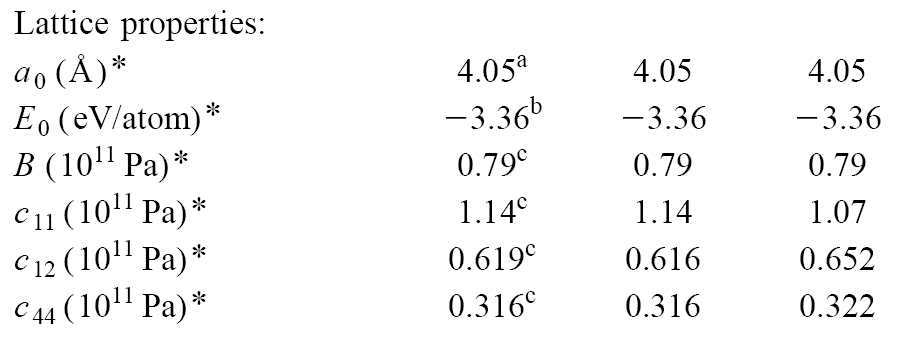
\includegraphics[width=1\textwidth]{Al_ref.PNG}
    \caption{Reference Value for FCC Al[4]}
\end{figure}

\begin{figure}[ht]
    \centering
    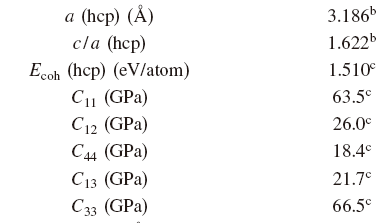
\includegraphics[width=0.9\textwidth]{Mg_ref.PNG}
    \caption{Reference Value for HCP Mg[5]}
\end{figure}

\begin{figure}[ht]
   \centering
   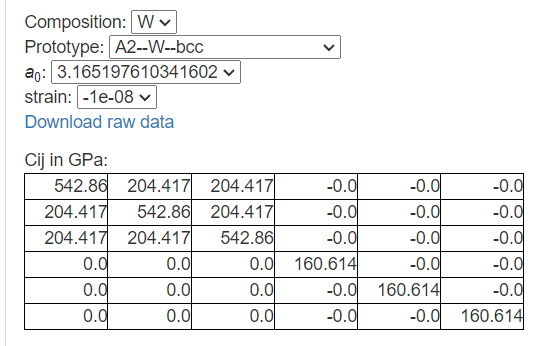
\includegraphics[width=1.1\textwidth]{W_ref.PNG}
   \caption{Reference Value for BCC W[6]}
\end{figure}
The reference values are provided in figure 4 to 6.
Thus, one could conclude that the simulated values of components of the elastic constant tensor for FCC Al, HCP Mg, and BCC W are generally agree with reference values.
Indeed, some error present. The reason could be the values of the lattice parameter used in LAMMPS are slightly different from their values in the reference paper.
\clearpage
For HEA, components of the elastic constant tensor are compared cross random lattice structures as shown in figure 4.
\begin{figure}[ht]
    \centering
    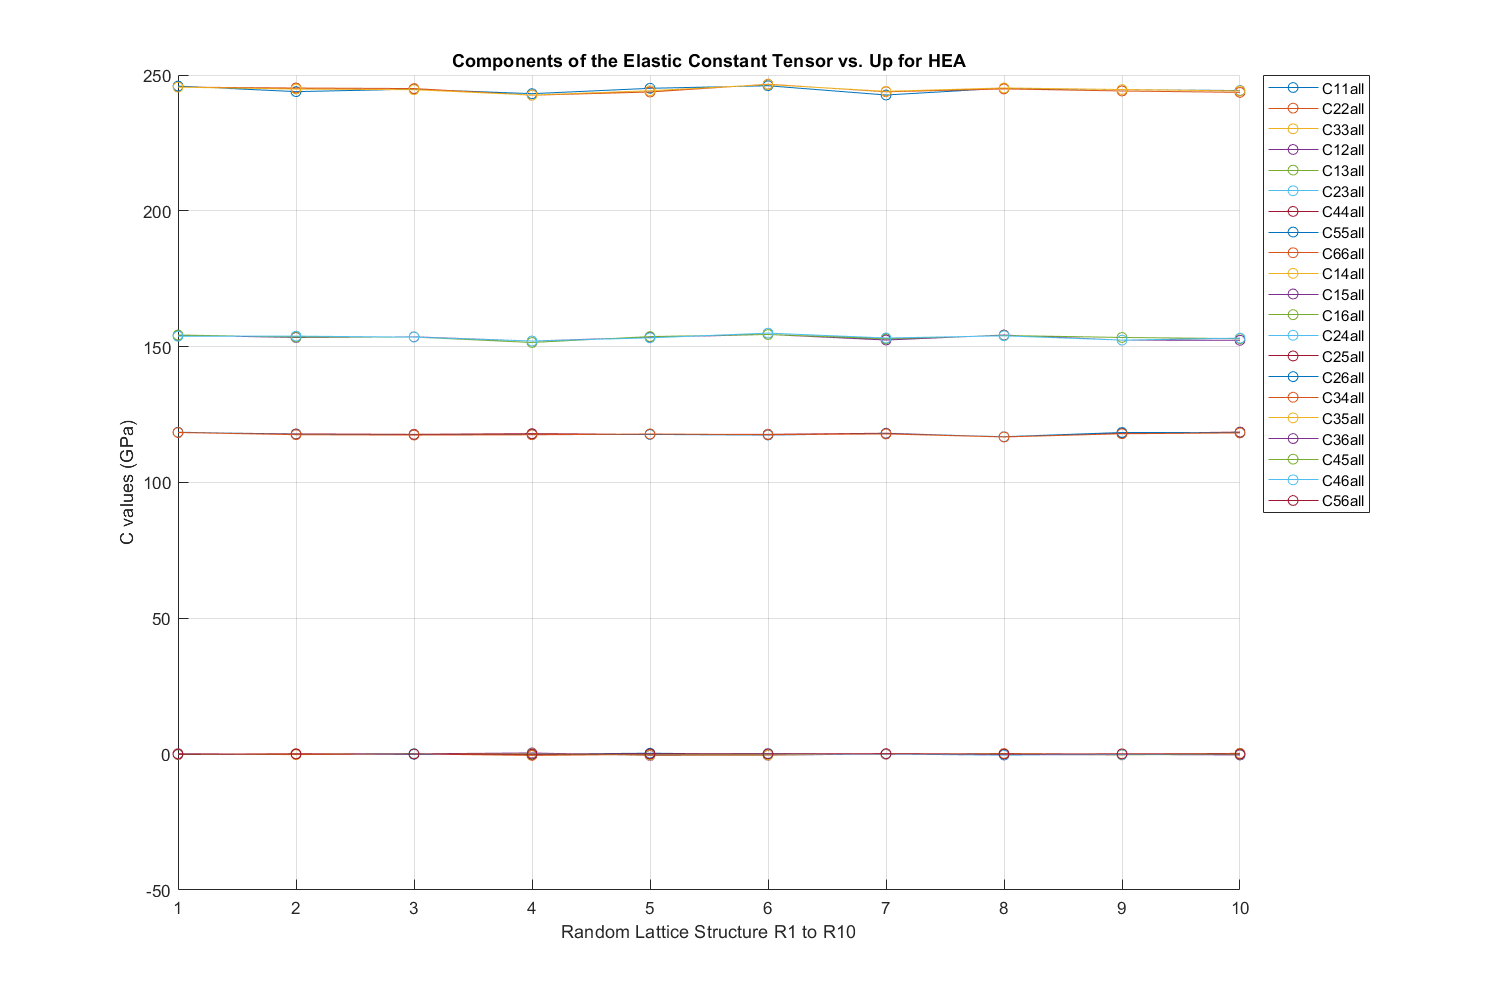
\includegraphics[width=1.1\textwidth]{HEA.png}
    \caption{Components of the Elastic Constant Tensor for HEA across Random Lattice Structures}
\end{figure} 
As we can see here, though the values are not always the same, they fluctuate in a relative small range shown in table 2, which indicates the consistence of the model.
And by comparing withe reference values shown in figure 8, one could conclude that the simulate elastic constant tensor values are generally reasonable.
\begin{table}[h!]
    \centering
    \begin{tabular}{|c|c|c|}
    \hline
    Parameter & Mean Value (GPa) & Max Percentage Difference (\%) \\ \hline
    \( C_{11all} \) & 244.555112 & 1.392473 \\ \hline
    \( C_{22all} \) & 244.509220 & 1.648953 \\ \hline
    \( C_{33all} \) & 244.625207 & 1.566594 \\ \hline
    \( C_{12all} \) & 153.273965 & 1.581219 \\ \hline
    \( C_{13all} \) & 153.445846 & 1.921851 \\ \hline
    \( C_{23all} \) & 153.429707 & 1.896058 \\ \hline
    \( C_{44all} \) & 117.888632 & 1.534806 \\ \hline
    \( C_{55all} \) & 117.815004 & 1.415642 \\ \hline
    \( C_{66all} \) & 117.733671 & 1.403118 \\ \hline
    \end{tabular}
    \caption{Mean values and maximum percentage differences of the \( C \) Values.}
    \label{table:c_parameters}
    \end{table}
    \begin{figure}[ht]
        \centering
        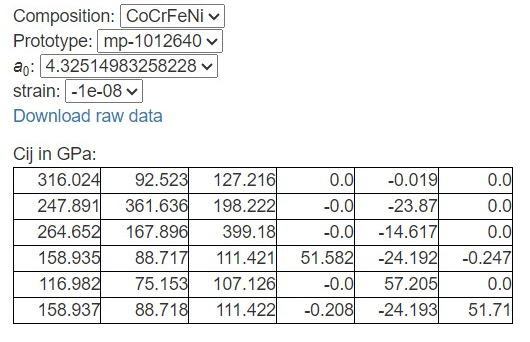
\includegraphics[width=0.9\textwidth]{HEA_ref.PNG}
        \caption{Reference Value for HEA[6]}
    \end{figure}

\clearpage
\section*{Conclusion}

This study successfully leveraged molecular dynamics simulations via LAMMPS to compute and analyze the elastic constant tensors for a variety of materials, including hcp-Mg, fcc-Al, bcc-W, and a novel high-entropy alloy (HEA) of Ni, Fe, Cr, and Co. Our findings reveal a remarkable consistency in the calculated elastic constants with known experimental and computational values, underscoring the robustness and accuracy of the simulation methodologies employed.

Particularly, the exploration into the HEA's elastic constants across different random lattice structures provides new insights into the material's mechanical properties, showcasing relatively minor fluctuations that indicate a stable and consistent behavior despite the alloy's complexity. This observation not only validates the computational model used but also opens up new avenues for the investigation of HEAs, which are of growing interest due to their potential applications in demanding environments.

Moreover, the systematic analysis of the convergence behavior of the elastic constants with varying finite difference displacement variables underscores the importance of simulation parameters in achieving accurate results. By optimizing these parameters, this work sets a foundation for future studies aiming to simulate and understand the mechanical properties of complex materials more efficiently.

Future work could expand upon this foundation by exploring a broader range of materials, particularly those with less conventional crystal structures or those used in cutting-edge applications. Additionally, the integration of more sophisticated simulation techniques and the exploration of temperature-dependent behaviors offer promising directions to further our understanding of material properties at the atomic level.


\section*{Reference}
[1]: Kittel, C. (2005). Introduction to Solid State Physics (8th ed.). Wiley.

[2]: Yoo, M. H., Lee, J. K., \& Nicholas, T. (1981). Slip, twinning, and fracture in hexagonal close-packed metals. Metallurgical Transactions A, 12(3), 409-418.

[3]: D. Farkas, and A. Caro (2020), "Model interatomic potentials for Fe–Ni–Cr–Co–Al high-entropy alloys", Journal of Materials Research, 35, 3031-3040. DOI: 10.1557/jmr.2020.294.

[4]: Mishin, Y., Farkas, D., Mehl, M. J., \& Papaconstantopoulos, D. A. (1998). Interatomic potentials for monoatomic metals from experimental data and ab initio calculations. Department of Materials Science and Engineering, Virginia Polytechnic Institute and State University, Blacksburg, Virginia 24061-0237; Complex Systems Theory Branch, Naval Research Laboratory, Washington, D.C. 20375-5345. ~Received 19 November 1997; revised manuscript received 26 August 1998!

[5]: Sun, D. Y., Mendelev, M. I., Becker, C. A., Kudin, K., Haxhimali, T., Asta, M., Hoyt, J. J., Karma, A., \& Srolovitz, D. J. (Year). Crystal-melt interfacial free energies in hcp metals: A molecular dynamics study of Mg. Journal Name, Volume(Issue), page range.

[6]: D R Mason et al 2017 J. Phys.: Condens. Matter 29 505501
\end{document}